\chapter{Experiment}

The \gls{caes} at the University of Melbourne has be assembled over a number of years. The experimental cycle can be divided into several parts which will be briefly descibed in this chapter. More details of the various experimental apparatus can be found in the group's recent papers \cite{bell_slow_2010, mcculloch_arbitrarily_2011, saliba_spatial_2012} and theses \cite{mcculloch_electron_2012, sheludko_shaped_2010, saliba_partially_2011}.


\section{Magneto-Optic Trap}

The first stage of the experiment is trapping rubidium atoms in a \gls{mot}. An oven is used to create Rubidium vapour with a temperature around 350K which is collimated and directed down the axis of the Zeeman slower. The Zeeman slower slows the atoms down such that when they reach the main chamber they can be trapped by the combined magnetic and optical traps.


\subsection{Rubidium Oven}

\begin{wrapfigure}{r}{0.5\textwidth}
\vspace{-80pt}
\centering
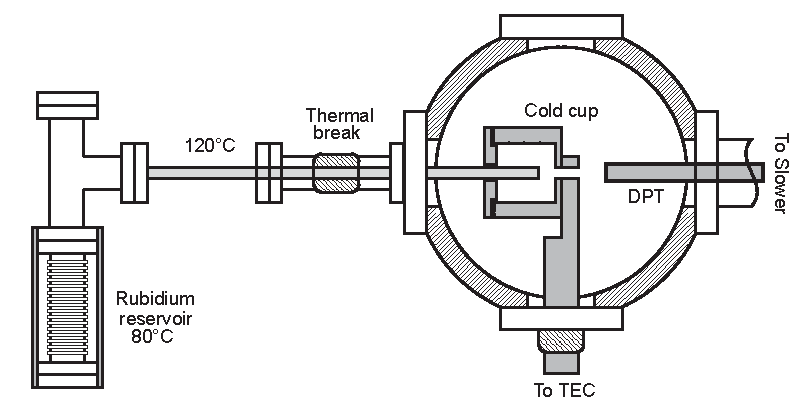
\includegraphics[width=0.48\textwidth]{figs/oven.pdf}
\caption{{\color{red} taken from Andy's thesis.} This figure shows the rubidium atom source.}
\label{fig:oven}
\end{wrapfigure}

Rubidium atoms in a reservoir are heated in an oven to approximately $80\,^{\circ}\mathrm{C}$. The resulting vapour effuses through a heated drift tube and is then incident on a `cold-cup'' aperture resulting in a collimated beam. At this point the atoms have a velocity in the region of 300m/s. This is shown in figure \ref{fig:oven}


\subsection{Zeeman Slower}
The Zeeman slower cools the atoms atoms from having a velocity of order 300m/s to 35m/s. This is achieved with doppler cooling using red-detuned light. As the atoms slow down the resonance condition changes so a magnetic coil with a tapered pitch is used to maintain the interaction. Another solution which is not implemented in this system is to use a frequency `chirp' in the cooling light.

An Eagleyards tapered amplifier seeded with light from two \glspl{ecdl} is used for the doppler cooling. The first \gls{ecdl} produces the cooling light and the second is used to repump any atoms that fall into a dark state.


    \subsection{Quasi-Mirror Magneto-Optic Trap}

Six beams etc. Near resonance. Magnetic field anti-Helmholtz.

\begin{figure}
\centering
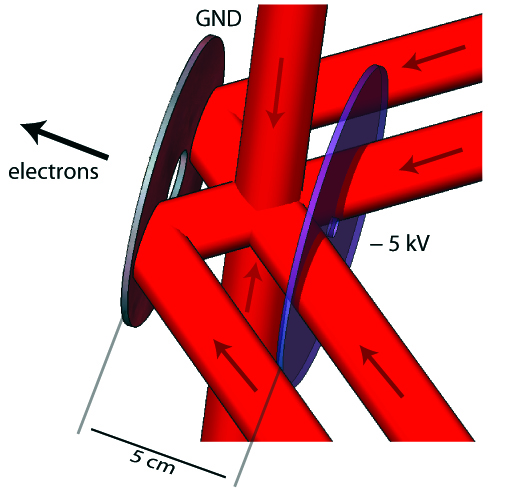
\includegraphics[width=0.45\textwidth]{figs/qMMOT.jpg}
\caption{{\color{red}Also taken from Andy's thesis.}}
\end{figure}

\section{Electron Generation}
text
    \subsection{Excitation}
text
        \subsubsection{ns}
text
        \subsubsection{fs}
text
    \subsection{Shaping}
text
    \subsection{Ionisation}
text
\section{Sample Chamber}
text
    \subsection{Beam Steering and Focussing}
text
    \subsection{magnetic tentacle monster}
text
    \subsection{Detector}
text
\section{Optical Dipole Trap}
text
    \subsection{TA}
text
    \subsection{Fiber laser}
text
    \subsection{dipole rig}
text
\section{absorption imaging}
text
\section{LabView}
text
